\documentclass{40k}

\begin{document}

\pagetitle{Cataclysm}

\begin{columns}

  \emph{Cataclysm} is an unofficial framework for team battles in
  Games Workshop's \emph{Warhammer 40,000}.  Most of it is loose
  guidelines for team organization, deployment zones, scheduling, and
  other logistical concerns external to the game.  Alongside that are
  a few game rules and clarifications for matches of multiple players
  and teams, and a default mission.  The framework is intended to
  serve as a basis for games ranging from a couple players fielding
  skirmish squads, up to mega-battles with many more players and
  massive armies.

%%------------------------------------------------------
\missionheading{Alliance}%

Each player is associated with an alliance, more or less working
together as a team.  The standard allies matrix and rules indicate how
players' armies interact within an alliance.  The number of players in
each alliance should be balanced but may vary slightly.

Each player nominates a warlord from their army as usual.  In
addition, each alliance must designate one of their warlords as their
warmaster.  These are simultaneously declared by the alliances
immediately after warlord traits are determined.

% However, all Come the Apocalypse pairs are treated as Desperate
% Allies, permitting an alliance to contain any faction.  The presence
% of Desperate Allies does not affect whether or not any units score or
% deny objectives.  Further, each army treats their own faction as a
% Battle Brother regardless of the matrix.

For large matches, a player from each alliance should act as commander
to lead and coordinate it.  Their primary tasks are communicating
logistics, rules, and the scenario to their team in advance, making
pre-game decisions such as allocating extra points or strategy cards;
and helping their team stay on time in the game itself.  Communication
and organization skills are more important for this role than tactical
prowess.  In large battles or when the alliance is trying to enact a
cohesive strategy, it may be helpful for the commander to release some
of their points to teammates and play a smaller army themselves.

%%------------------------------------------------------
\missionheading{Army Selection}%

Cataclysm army lists are selected according to the standard rules and
any external constraints imposed by the organizer(s), such as campaign
requirements.  If alliances can coordinate in advance, unique units
and wargear might be required to be unique across an alliance's entire
combined force.  For pick-up style events, however, unique items
should be simply either banned entirely or permitted without
restriction.

To keep planning simple, each player should be granted an equal number
of points rather than trying

\columnbreak
\noindent
\begin{minipage}[h]{1.0\linewidth}\centering\small\it%
\fbox{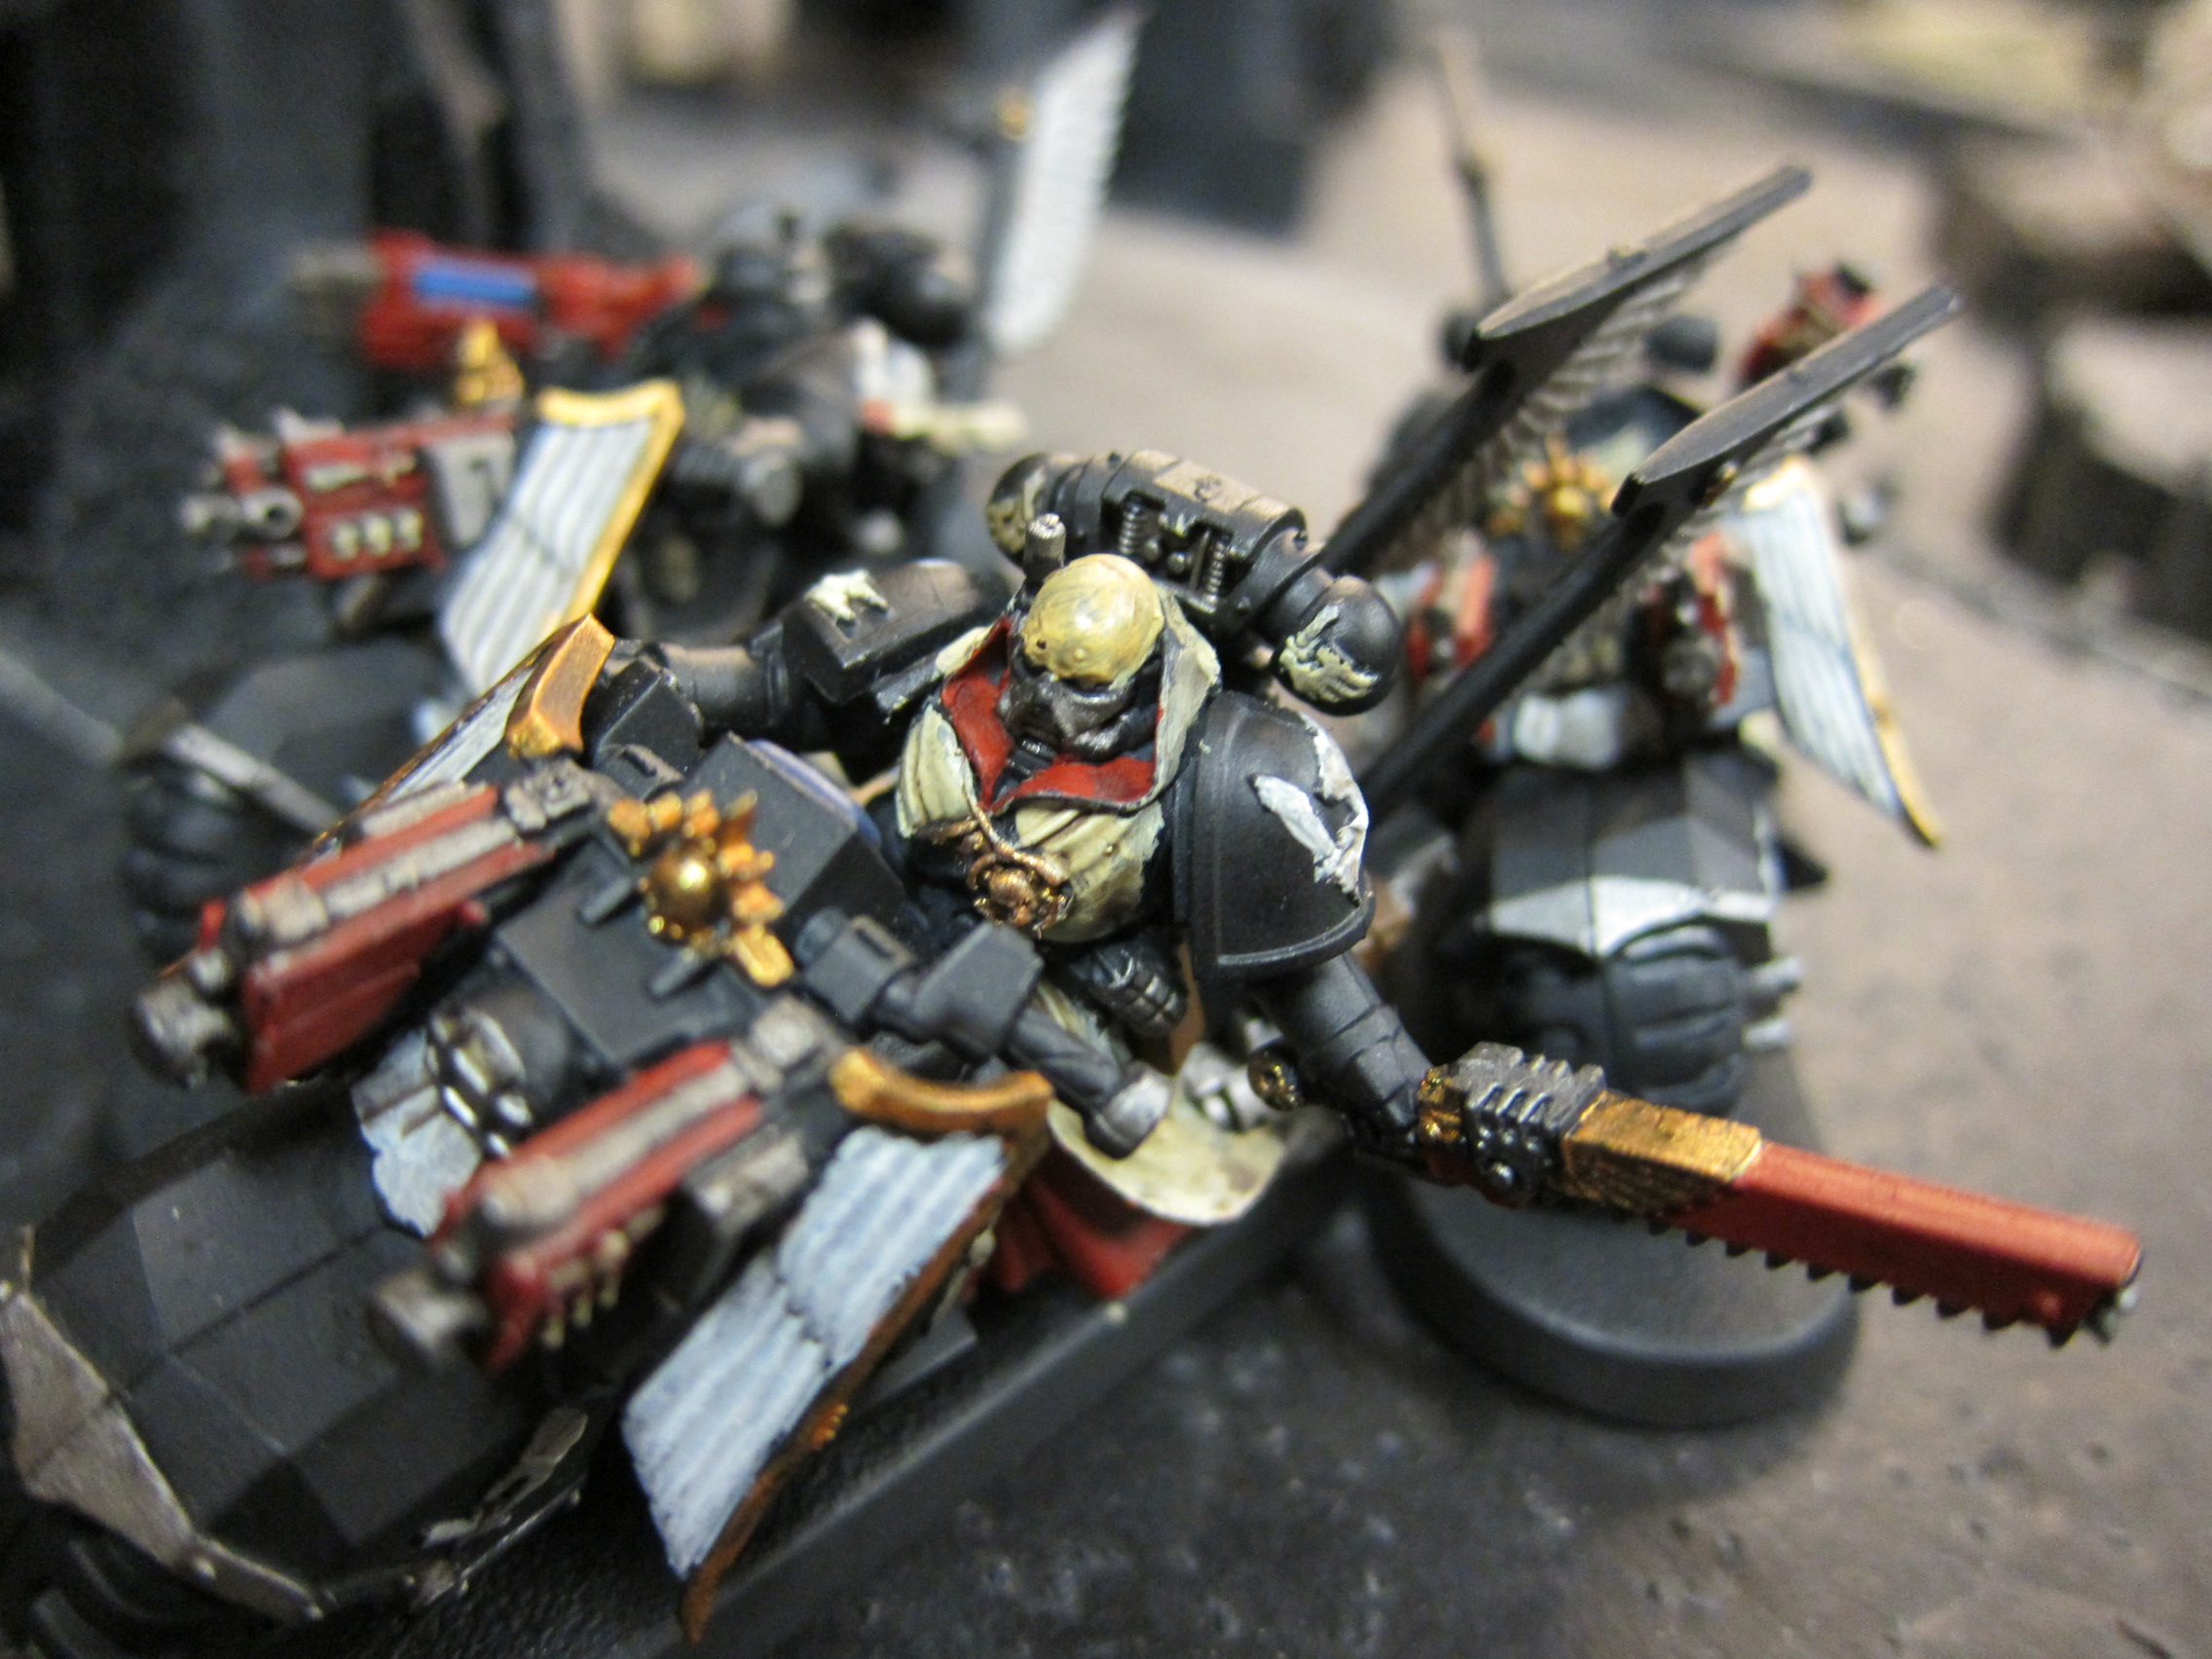
\includegraphics[width=(1.0\linewidth)]{pics/biker-sergeant}}\\
Come the apocalypse on our wings!
\end{minipage}
\smallskip

\noindent to divide a fixed amount per alliance.  Alliances with fewer
players than the largest should allocate additional points among their
players, in any fashion they wish, to match that greater total.  With
large armies players may also be allocated more points to cover for
those with fewer models.  Players should bring extra models to enable
these balancing additions.  For large games the commanders should
coordinate this in advance as best as possible, but the teams and
organizer(s) should always be prepared for no-shows.



In this framework the following shorthand is used to roughly classify
matches by the points per player:

\bigskip
\centerline{\begin{tabular}{cr}
  \textbf{Mini} &  500+ points\\
  \textbf{Classic} & 1000+ points\\
  \textbf{Apocalyptic} & 2000+ points\\
\end{tabular}}

%%------------------------------------------------------
\missionheading{Schedule}%

For larger and more organized events it is important to fully utilize
the available time, as well as to not run over time or have to end the
battle prematurely.  Keeping a large number of players on track
in-game can also be a significant challenge.  Cataclysm missions
should therefore run for a fixed~5 or~6 turns, determined in advance.
Based on the number of turns, the organizer(s) should establish and
enforce a detailed schedule.  Schedules should incorporate setup and
cleanup, food and other breaks, deployment, and a breakdown by turn.
Notably, later turns generally play faster and can be assigned less
time as players find their rhythm and have fewer models left.
\end{columns}

\pagebreak

\begin{examples}{Sample Schedules}
  
\begin{columns}
\centerline{\bf Mini or Classic,~3 Alliances,~5 Turns}

\centerline{%
\begin{tabular}[t]{rl}
30 min & Set up tables \& terrain\\
45 min & Deployment (up to~15 min each)\\
45 min & Turn 1 (15 min per alliance)\\
45 min & Turn 2\\
45 min & Turn 3\\
30 min & Turn 4 (10 min per alliance)\\
30 min & Turn 5\\
30 min & Pack up\\
\\
\end{tabular}%
}

\centerline{5 hours total}

\columnbreak

\centerline{\bf Apocalyptic,~2 Alliances,~6 Turns}

\centerline{%
\begin{tabular}[t]{rl}
60 min & Unpack, set up tables \& terrain\\
60 min & Deployment (up to~30 min each)\\
110 min & Turn 1 (55 min per side)\\
30 min & Lunch\\
110 min & Turn 2\\
100 min & Turn 3 (50 min per side)\\
100 min & Turn 4\\
30 min & Dinner\\
90 min & Turn 5 (45 min per side)\\
90 min & Turn 6\\
60 min & Pack up and clean up\\
\end{tabular}%
}

\smallskip
\centerline{14 hours total (!)}

\end{columns}
\end{examples}


\begin{columns}


%%------------------------------------------------------
\missionheading{Tables and Deployment Zones}%

Tables should be 4--6' across on the short axis, proportional to army
sizes.  Any smaller and assumptions about first turn assaults and
other game aspects begin to break down.  Any larger and many armies
will struggle to make contact, in addition to being physically
difficult to reach across.  Generally long axis table edges should
be~2--4' per player in an alliance, or roughly equivalently~1'
per~750--1500 points on a side.  Additional room is needed for the
players to move around, as well as supporting table space depending on
the size of the armies.  An extended article on table sizes for large
games is available here:

\smallskip
\centerline{\small\url{http://bit.ly/15PRQRX}}

\smallskip%
Deployment zone geometry necessarily varies with the number of
alliances, players, army sizes, and available table space.  These must
be planned in advance by the organizer(s).  Zones should all be
equally sized, with roughly~2 square feet per~1000 points in the
alliances, and roughly the same shape.  With four alliances it might
not be practical for zones to all be adjacent to each other.
Critically though, each zone should be as close to~24'' from its
neighbors as is feasible to preserve a number of fundamental
assumptions about assault, shooting, and mobility ranges.  A specific
table edge or segment of an edge should be identified for each
alliance for purposes of reserves, falling back, and other mechanics.

\vfill\hbox to 0pt{}

\columnbreak

\missionheading{Startup and Turn Order}%

The match begins by players determining warlord traits, psychic
powers, and other pre-game effects.

Each alliance then simultaneously makes a bid for deployment time and
turn order, given as a whole number of minutes up to a maximum by game
size:

\smallskip
\centerline{\begin{tabular}{cr}
  Mini &  10 minutes\\
  Classic & 20 minutes\\
  Apocalyptic & 30 minutes\\
\end{tabular}}

\bigskip%
Each alliance is given as many minutes to deploy as they bid.  Any
units or models not deployed when time runs out automatically go into
Strategic Reserve.

The order of bids from lowest to highest is the order by which
deployment zone selection, placement of objective markers, deployment,
and game turns are respectively performed, in that sequence.  Note
that this is not the standard \emph{Warhammer~40,000}~7th edition
startup order.  Ties on bids are broken with a roll-off.  Seize the
Initiative is not applied.


\missionheading{Turns}

Each player in an alliance simultaneously takes actions as usual in
its turn, with any order of activated units.  Alliance turns are
player turns in all ways.

In game terms, players in an alliance conduct all their actions within
a phase simultaneously and then move on to the next phase together
synchronously. However, in practice, players with no more actions to
take in a phase should carefully proceed to the subsequent phase,
provided there is no effect on another player's remaining actions in
the current phase.

Importantly, time must be specifically reserved in each alliance turn
for ongoing combats.  Otherwise assault oriented armies and units are
short-changed by not having these fights play out as often as they
should, penalizing their damage output and mobility.  The organizer(s)
and commanders must monitor whether or not this is necessary in each
turn and enforce the following minimum assault phase if so:

\smallskip
\centerline{\begin{tabular}{cr}
  Mini &  5 minutes\\
  Classic & 10 minutes\\
  Apocalyptic & 15 minutes\\
\end{tabular}}

\smallskip%
Teammates already finished their turn should help resolve ongoing
combats if a player with units engaged in combat is still moving or
shooting.  Otherwise the engaged player must move on to assault with
their other phases left unfinished.

Any actions not completed within turn time limits are simply
forfeited.  Once in the course of the game an alliance can extend
their current turn by~5 minutes.


%\vfill
%\bigskip
%\begin{story}{7pt}{Thought for the Day}
%Serve the Emperor, serve thyself.
%\end{story}

\missionheading{Scope Limits}

Special rules that affect all units, all enemy units, or the entire
table are not applied.  Specific examples include the Chaos Daemons'
Warp Storm table, the Lord of the Storm rules for the Necron's Imotekh
the Stormlord, and the Necron Solar Pulse, none of which take effect.
This does not include Cataclysm effects imposed by the mission or
organizer(s).

Army-wide buffs apply only to that detachment of that player's forces,
as in a usual game, regardless of other factions that may be present
their alliance.  For example, nominating Vulkan He'stan as a warlord
makes only that player's Melta weapons in Vulkan's detachment
Mastercrafted and does not affect any other detachments or players in
their alliance, including other Salamanders Space Marines.

\missionheading{Psychic Phase} 

A single~D6 is rolled by the current alliance in the psychic phase to
determine the base warp charge to be used by all players, who
otherwise follow the standard rules to generate their own distinct
warp charge pools.  Each alliance with fewer players than the largest
alliance receives an additional base amount of charge for each player
fewer on their team, allocated to their players however they wish.

Players may only cast and deny powers using their own warp charge.
The single player from any opposing alliance with any model within
48'' of a psyker casting a power and willing to use the most warp
charge to attempt denying a successful spell may do so.  If multiple
players want to attempt denying, select one randomly.  Note that
players may attempt to deny spells targeted at models other than their
own.


\missionheading{Shooting Phase}

Players may shoot into ongoing close combats that do not include any
units from their alliance, targeting the combat as a whole.  Blast
templates scatter as usual and hits are allocated to units for each
model under the template.  Other hits are allocated to the closest
model in sequence as usual, which may mean that multiple units are
hurt as models are removed.

After resolving wounds, the units in combat are assumed to be still
locked in that combat unless all the models of an alliance have been
eliminated, even if the units are no longer in physical contact due to
removed casualties.  Consolidation moves are not made if an alliance
is eliminated.  Units shot at in combat do not take morale checks at
the end of shooting.

\vfill
\noindent%
\begin{minipage}[h]{1.0\linewidth}\centering\small\it%
\fbox{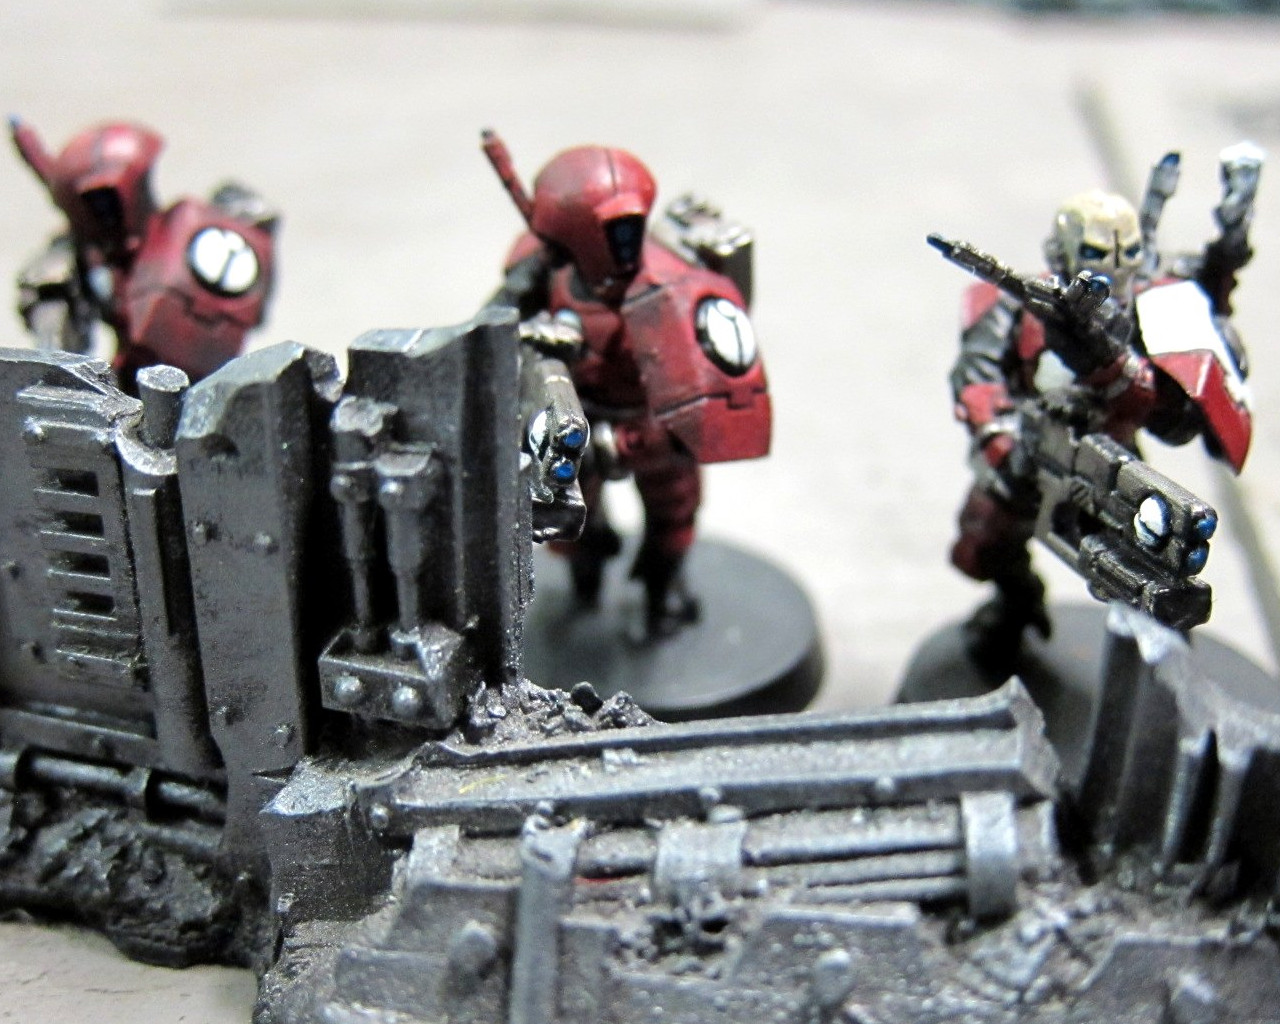
\includegraphics[width=(1.0\linewidth)]{pics/tau-line-cropped}}\\
Firing solution on coordinates alpha alpha nine six four!
\end{minipage}

\end{columns}

\vfill
\begin{story}{0.35in}{The Greater Good}
  Shas'ui Ke'ssai crouched low behind the crude rubble barricade.  His
  hooves trembled with the clamorous approach of the humans' ugly,
  stinking, smoking vehicles.  In that moment, he realized he hated
  them.  He hated them for their violence, and he hated them for what
  they'd done to his world.  But most of all, he hated them for
  teaching him to hate.
\end{story}

%%------------------------------------------------------
\pagebreak
\begin{columns}


\missionheading{Assault Phase}

In the assault phase, the alliances alternate selecting combats to be
resolved beginning with the currently active team.  This ensures the
current team cannot solely resolve their preferred combats before time
runs out for the turn.  In game terms, assaults are resolved in order
one-by-one, as usual. In practice, assaults that cannot affect each
other should be resolved simultaneously as possible.

Units may charge as usual into ongoing close combats including units
from multiple other alliances.  Combats are resolved in the assault
phase of each alliance with engaged units, making combats with more
than two alliances particularly deadly!

\missionheading{Apocalyptic Reserves}

In apocalyptic games, units placed into Strategic Reserve arrive
according to the following schedule rather than rolling each turn as
per the standard rules:

\smallskip \centerline{\begin{tabular}{cp{2.5in}}
    Turn 1 & Zooming flyers \& deep striking units\\
    Turn 2 & Any unit capable of moving~12'' or more in a single
             movement phase, e.g., beasts and vehicles, including
             transports with embarked units\\
    Turn 3 & All other units\\
\end{tabular}}

\smallskip%
Once per game any unit, wargear, fortification, or other special rule
that can manipulate reserve rolls may be used to shift the scheduled
arrival of a unit by one turn.  This may be applied to friendly or
enemy units and may shift them up or down as appropriate to the
original ability's rules and modifiers.  No unit may be affected in
such a way more than once per game, and no unit may be delayed past
Turn~3.

For example, an Astra Militarum Fleet Officer could delay the arrival
of an opposing Heldrake until Turn~2.  That Fleet Officer cannot then
delay or advance another unit for the remainder of the game.  A second
Fleet Officer or another unit also could not delay that same Heldrake
again to Turn~3.

\end{columns}

%%------------------------------------------------------
\missiontitle{Cataclysm Mission: Hold and Repel}

\begin{columns}

  This is a good default mission template for Cataclysm games that
  works well for any number of alliances.

  \missionheading{Table Setup}

  After determining deployment zones, place primary objective markers.
  First, each alliance in turn order places one home objective in its
  deployment zone.  Each then in turn places one target objective in
  the adjacent deployment zone clockwise around the table.  Finally,
  each alliance in turn then places one neutral objective in no
  alliance's deployment zone.  Objective marker placement follows all
  standard rules.

  \missionheading{Game Length}

  Settle beforehand on~5 or ~6 turns and a schedule.

  \missionheading{Mission Specific Rules}

  \vspace*{-9pt}%
  \missionsubheading{Reserves.} As on page~135 of the main rulebook
  and modified by Cataclysm rules for apocalyptic matches.

  \missionsubheading{Nightfighting.} On a~D6 of~4+ before the first
  alliance begins its first turn, all units have Stealth for Turn~1.

  \missionheading{Scoring} 

\vspace*{-9pt}
  \missionsubheading{Primary Objectives.}  Control of primary
  objective markers is cumulatively scored at several points based on
  the predetermined game length:

  \smallskip%
  \begin{tabular}{cl}
    5 turns & After the~1st,~3rd, and~5th turns\\
    6 turns & After the~2nd,~4th, and~6th turns\\
  \end{tabular}

  \smallskip%
  The value of each marker varies by its location relative to the
  alliance controlling it:

  \begin{squishitemize}
  \item Primary objectives in the next enemy deployment zone clockwise
    around the table are worth +3 victory points each.

  \item Primary objectives in the alliance's own deployment zone are
    worth +2 victory points each.

  \item All other primary objectives are worth +1 victory point each.
  \end{squishitemize}

  \missionsubheading{Secondary Objectives.}  The following secondary
  objectives award additional victory points to each alliance at the
  end of the game:
  \begin{squishitemize}
  \item +2 for each enemy warmaster directly forced to be removed as a
    casualty by the alliance;

  \item +1 for each enemy warlord directly forced to be removed as a
    casualty by the alliance, not including warmasters;

  \item +1 for each enemy deployment zone in which the alliance has a
    scoring unit;

  \item +1 if there are no enemy models, scoring or otherwise, in the
    alliance's own deployment zone.
  \end{squishitemize}

  \bigskip%
  The alliance with the most victory points emerges triumphant from
  the Cataclysm!

\end{columns}

\divider

\begin{columns}

\missionheading{Disclaimer}%

Cataclysm is completely unofficial, unauthorized, and unaffiliated
with Games Workshop.

\smallskip{\footnotesize Adepta Sororitas, Adeptus Astartes, Astra
  Militarum, Blood Angels, Chaos Daemons, Chaos Space Marines, Dark
  Angels, Dark Eldar, Eldar, Grey Knights, Necrons, Orks, Space
  Wolves, Tau Empire, Tyranid, Forge World, Games Workshop, Warhammer,
  and all associated marks, names, races, race insignia, characters,
  vehicles, locations, units, illustrations, images, and models from
  the Warhammer 40,000 universe and game are either \textregistered,
  TM, and/or \textcopyright\ Copyright Games Workshop Ltd 2000--2014.
  Used without permission, no challenge to status intended, all rights
  reserved to their respective owners.}

% variably registered in the UK and other countries.

% All Games Workshop marks and terms have been used without
% permission; no challenge to their status is intended.  All rights
% are reserved to their respective owners.

%%----------------------------------------------
\columnbreak
\missionheading{Credits}%

\smallskip\noindent {\bf Design:}
\begin{minipage}[t]{3in}
The Philadelphia Area Gaming Enthusiasts\\
\centerline{\url{http://pagegaming.com/}}
\end{minipage}

\smallskip\noindent{\bf Text, Photos, and Typesetting:} Joe Kopena

\smallskip\noindent This PDF has been produced using solely open source
tools: Emacs, \LaTeX, Inkscape, and GIMP.

%%----------------------------------------------
\missionheading{Version}%

\noindent This is \emph{Cataclysm} \today.

\vfill

\hbox to 0pt{}

\end{columns}

\begin{tikzpicture}[remember picture, overlay]%
    \node[inner sep=0pt,above left,xshift=1.75cm,yshift=1.7cm] at (current page.south east) {%
        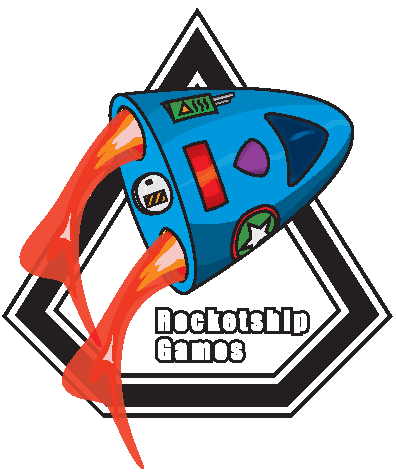
\includegraphics[width=1.5in]{art/rocketshipgames-logo}%
    };%
\end{tikzpicture}

%\begin{tikzpicture}[remember picture, overlay]
%  \draw [fill=white,draw=none] (current page.south west) rectangle (2,0.25) ;%
%\end{tikzpicture}

\begin{tikzpicture}[remember picture, overlay]
  \node[above=72pt,xshift=1in,draw=none,text centered] at (current page.south) {%
    \scalebox{2}{{\sf\Large\bf rocketshipgames.com}}%
  };%
\end{tikzpicture}

\end{document}

%%------------------------------------------------------
\pagebreak
\missionheading{Deployment Configurations}%

%%{\parfillskip0pt\relax\par}

